%%%%%%%%%%%%%%%%%%%%%%% file template.tex %%%%%%%%%%%%%%%%%%%%%%%%%
%
% This is a general template file for the LaTeX package SVJour3
% for Springer journals.          Springer Heidelberg 2010/09/16
%
% Copy it to a new file with a new name and use it as the basis
% for your article. Delete % signs as needed.
%
% This template includes a few options for different layouts and
% content for various journals. Please consult a previous issue of
% your journal as needed.
%
%%%%%%%%%%%%%%%%%%%%%%%%%%%%%%%%%%%%%%%%%%%%%%%%%%%%%%%%%%%%%%%%%%%


\RequirePackage{fix-cm}
%
%\documentclass{svjour3}                     % onecolumn (standard format)
%\documentclass[smallcondensed]{svjour3}     % onecolumn (ditto)
%
%\documentclass[smallextended]{svjour3}       % onecolumn (second format)
\documentclass[twocolumn]{svjour3}          % twocolumn
%
\smartqed  % flush right qed marks, e.g. at end of proof
%
\usepackage{graphicx}
\usepackage[spanish]{babel}
% \usepackage{mathptmx}      % use Times fonts if available on your TeX system
%
% insert here the call for the packages your document requires
%\usepackage{latexsym}
% etc.
%
% please place your own definitions here and don't use \def but
% \newcommand{}{}
%
% Insert the name of "your journal" with
\journalname{Autonomous Robots}
%
\begin{document}

\title{Jderobot open source framework for robotic, computer vision and home automation applications
%\thanks{Grants or other notes
%about the article that should go on the front page should be
%placed here. General acknowledgments should be placed at the end of the article.}
}
%\subtitle{Do you have a subtitle?\\ If so, write it here}

%\titlerunning{Short form of title}        % if too long for running head

\author{José M. Cañas \and David Lobato \and Roberto Calvo \and Julio Vega \and Eduardo Perdices \and Francisco Rivas}

%\authorrunning{Short form of author list} % if too long for running head

\institute{F. Author \at
              first address \\
              Tel.: +123-45-678910\\
              Fax: +123-45-678910\\
              \email{fauthor@example.com}           %  \\
%             \emph{Present address:} of F. Author  %  if needed
           \and
           S. Author \at
              second address
}

\date{Received: date / Accepted: date}
% The correct dates will be entered by the editor


\maketitle

\begin{abstract}
For a given robot most of its intelligence lies on its software, the way it coordinates its sensing and actuation capabilities. In the last years several frameworks have appeared that simplify and speed up the development of robot applications. They favor the code reuse and take benefits from modern software engineering tecniques. This paper presents the open source robotics framework Jderobot, a distributed and component oriented platform. It uses explicit interfaces among components and ICE as communication middleware. It provides many tools for robot programming like a template for robot control components, visual HFSM creation, etc. Several examples of research and applications done with this framework are also described as experimental validation of it.
\keywords{Robot software \and Second keyword \and More}
% \PACS{PACS code1 \and PACS code2 \and more}
% \subclass{MSC code1 \and MSC code2 \and more}
\end{abstract}

\section{Introduction}
\label{intro}

%software importance
Most of robot intelligence lies on its software. Once the robot sensor
and actuator devices are set, the robot behavior is fully caused by
its software. There is no universally accepted way of programming
robots. Regarding the language, there are robots programmed in assembler, in C and C++ or in Java. 

The importance of good programming practices has increased in last years. Code reuse to avoid restart from scratch for every new robot. JOSER, ieee chapter, autonomous robots special issue. Software engineering.

Encapsulating robot capabilities in functions is a slippery issue as behaviors usually don't fit into the functional abstraction where the caller invoques the function and stops it flow of execution until receives the function response or output.

Simulators are useful tools in robotics.

Operating systems and robotic frameworks.

% software requirements in robotics
Compared with other computer science fields the development of robot applications exhibits some specific requirements. First, liveliness and real-time processing: software here has to take decisions with in a fast way, for instance in robot navigation or image processing. Second, robot software has to deal with multiple concurrent sources of activity, and so tends to be multitask. Third, computing power is usually distributed along several connected computers, and so the robotic software may be distributed. Fourth, the robotic software typically deals with heterogeneous hardware. New sensor and actuator devices continually appears in the market and this makes maintenance and portability to new robots or devices more complex. Fifth, the robotic software usually includes a Graphical User Interface, mainly for debugging purposes. Sixth, the robotic software should be expansible for incremental addition of new functionality and code reuse.

% robotic frameworks 
Mobile robot programming has evolved significantly in recent years, and two approaches are currently found. On one hand, application programs for simple robots obtain readings from sensors and send commands to actuators by directly calling functions from the drivers provided by the seller. On the other hand, we have identified many common features across commercial and non-profit robotic frameworks SDKs.

First, they offer a simple and more abstract access to sensors and actuators than the operating systems of simple robots. For example, in a Pioneer with a laser rangefinder, the applications can obtain readings using ARIA or directly through a serial port. Using ARIA, one need only invoke a method and ARIA will take charge of refreshing the variables. Using the operating system directly, the application must request and periodically read the data from the laser through the serial port, and must identify the protocol of the
device to compose and analyze the low level messages correctly. The abstract access is also offered for actuators.

Second, the software architecture of the SDK sets the way the application code obtains sensor data, commands the motors, or uses a developed functionality. There are many software options: calling to library functions, reading variables, invoking object methods, sending messages via the network to servers, etc.. Depending on the programming model the robot application can be considered an object collection, a set of modules talking through the network, an iterative process calling to functions, etc.

Third, usually the SDK includes simple libraries, tools and common use functionality, such as robust techniques for perception or control, localization, safe local navigation, global navigation, social abilities, map construction, etc. The robot manufacturers sell them separately or include them as additional value with their own SDK. For example, ERSP includes three packages in the basic architecture: one for interaction, one for navigation and another for vision. There are several advantages of using the SDKs. First, they favor the portability of applications between different robots. Second, they promote code reuse, shortening the development time and reducing the programming effort needed to code the application as long as the programmer can build the program by reusing the common functionality, keeping herself focused in the specific aspects of her application. And third, the software architecture offers a way to organize code, allowing the handling of code complexity when the robot functionality increases.

% our proposal
We present our open-source robotic software framework, named Jderobot (http://jderobot.org), which is component oriented, uses ICE as communication middleware and includes several useful tools and libraries. Several sensor and actuator drivers have been programmed or reused from the open-source community. This framework has been widely used in our group for research and teaching for more than eight years. Jderobot has been designed for scenarios with sensors, actuators and intelligent software in between. The typical scenario is robotics, but also computer vision and home automation.

% open source
Why open-source in robotics? First, it provides independence of robot manufacturers and so it may support robots from different companies. Using open-source you are free to modify, debug, or improve the software, so the final software quality is high and does not depend on a company. One strong motivation is also the feeling of contributing to the robotics community and to return the favor. We have extensively used open-source libraries and tools in our research (OpenCV, Gazebo, GTK, etc.). Research algorithms can be replicated easily and compared with standard tools. The tools must be open in order to trust in them.

% paper organization
This paper is organized as follows. The state of the art in robotic
frameworks fills section \ref{sec:relatedworks}, where other platforms
are briefly presented. Section \ref{sec:jderobot} fully explains the
proposed platform, the ideas behind its design, the set of standarized
interfaces and developed drivers and the tools included to make the
development of new applications easier. In section \ref{sec:research} some successful examples using Jderobot are presented, both in research and in teaching. Finally conclusion section summarizes the main remarks.

\section{Related works}
\label{sec:relatedworks}

Robotic frameworks can be grouped in two main paradigms, those tighly
coupled with a cognitive model in their designs and those designed
just from a pure engineering criteria. The first ones \textit{force}
the user to follow a set of rules in order to program certain robotic
behavior, while the second ones are just a collection of tools that
can flexibly be put toguether in several ways to acomplish the task.

%cognitive frameworks
Cognitive robotic frameworks were popular in the 90s and they were
strogly influenced by the AI, where planning was one of the main
keys. Indeed one of the strenghts of such frameworks were their
planning modules built around a sensed reality. A good example of cognitive
frameworks was Saphira \cite{konolige98} based on a behaviourist
cognitive model. Some of its low-level functionality was rewriten as a
C++ library called ARIA \cite{aria} that it's still suplied with the
popular robotic platforms from MobileRobots/ActivMedia.

%current frameworks
Current robotic frameworks focus their designs on the requirements
that robotics applications need and let the user (the programmer) to
choose the organization that better fits with her specific
application. Main requirements driving the designs are: multi-tasking, distributed, easy to
use and code reusability. Another requirement, we belive it's a main
key, it's the open source code, that creates a synergy between the use
and the developer. Proof of this is the two most popular robotic
frameworks in the last years: PlayerStage
\cite{Gerkey03,collet05,vaughan2007} which has been the \textit{standard de
facto} in most of the last decade and ROS \cite{quigley09} which is
taking the place currently.

%key achivements
Key achivements of modern frameworks are the hardware abstraction, hiding the complexity of accesing heterogeneous hardware (sensors and
actuators) under standard interfaces, the distributed capabilities
that allows to run complex systems spread over a network of computers,
the multi-platform and multi-language capabilities that enables the
user to run her software in multiple architectures, and the existence
of big communities of software that share code and ideas.

%examples
Main examples of modern frameworks are the aformentioned PlayerStage
and ROS. The first has two main parts, Player, provides a network
interface to the robot hardware through a collection of standard
interfaces. This standard interfaces are implemented by drivers, one
for each different hardware. This way a user only needs to know the
standard way to use, let say, a laser ranger and not every different
brand. The second part is Stage, a 2D simulator that allows the user
to try in a simulated world before trying on a real platform. In
addition to this, PlayeStage framework provides a variety of
algorithms that are used with the same concept through standard
interfaces. Other example is ROS that employs the same concept of
standard interfaces with the addition of a middleware that greatly
simplifies the network distribution. The core system of ROS comes with
a collection of tools to help with tasks as project management, system
debugging and centralized logging. Currently has a growing community
and its site hosts a great collection of hardaware drivers, algorithms
and other tools.

Another important example is ORCA \cite{brooks05,brooks07} based on the
same concepts mentioned, but with the idea of expending less effort
building the underlying middleware elements . This way they chose to
use Ice from ZeroC \cite{henning04}, a powerful object oriented middleware
that allows them to focus in the robotic problems.

%%CARMEN \cite{montemerlo03}
%%ROS, ORCA, Miro, RoboComp, Aria, 
%%Microsoft Robotics Studio, Beesoft. ERSP.

\section{Jderobot platform}
\label{sec:jderobot}

Some history. Keep away the cognitive ideas, focus on software
architecture. Nace como implementación de arquitectura cognitiva,
tesis doctoral jdec \cite{canas02}. Evolucionó a una plataforma de programación para
aplicaciones robóticas, domóticas y de visión computacional (sensores,
actuadores, inteligencia).



\begin{itemize}
\item Orientada a componentes distribuidos y multilenguaje
\item La mantiene un grupo de desarrolladores, es abierta
\item {http://jderobot.org}, manuales, descarga, ejemplos
\end{itemize}
Software libre (licencia GPLv3), paquete debian


Arquitectura cognitiva JDE:
\begin{itemize}
\item Comportamiento = {percepción} y {control}
\item Fragmentación en unidades asíncronas concurrentes (esquemas)
\begin{itemize}
\item[-] de percepción elaboran estímulos
\item[-] de actuación toman decisiones
\end{itemize}
\item La colección de esquemas se organiza en \textit{jerarquía} dinámica (JDE)
\item Sigue el paradigma basado en comportamientos
\end{itemize}

Arquitectura cognitiva: Esquemas.
Un {esquema} es un flujo de ejecución independiente, con un objetivo
\begin{itemize}
\item Funcionamiento continuo
\item Se puede activar y desactivar a voluntad
\item Modulable a través de parámetros
\item Su funcionalidad se usa despertándolo y modulándolo
\item {Perceptivos}: producen estímulos (piezas de información) y los mantienen actualizados. Lecturas sensoriales, transformaciones más elaboradas 
\item {Actuación}: toman decisiones para conseguir o mantener un objetivo, comandos a los actuadores o la activación y modulación de otros 
\end{itemize}



\subsection{Software architecture design}

Some history and lessons learnt: 4.3. 

Threads. GUI specific interface. 

\begin{itemize}
\item Component oriented 
\item Iterative execution
\item Concurrent and optional visualization
\item Processes better than threads
\item ICE for communication
\item Explicit standard interfaces
\item Configuration files 
\end{itemize}

multilanguage, distributed intermachine, Android, efficient

Reuse other open-source libraries: OpenCV, Gearbox, GTK, PCL, OpenGL, PlayerStage, Gazebo, GSL, Cwii.


GUI thread separated from control thread.
Iterative control, iterative perception. Component frequency.
Standard interfaces for communication with other components.

Modelo de programación: Componente
\begin{itemize}
\item Cada esquema se materializa en un {componente} software 
\item El funcionamiento continuo como {ejecución iterativa}, iteraciones periódicas a cierto ritmo para percibir o para actuar
\item Ofrece funcionalidad y usa la de otros a través de {interfaces} explícitos
%el componente es la unidad básica
\item Aplicación $=$ conjunto de componentes concurrentes que interoperan
\item {Multimáquina} y {multilenguaje}: C, C++, python, Java... 
\item Usa el middleware de comunicaciones ICE (zeroC)
\end{itemize}

Ejecución iterativa:
\begin{itemize}
\item Iteración de control o de percepción
\item component\_cycle 
\item \texttt{gettimeofday}
\item \texttt{usleep}
\item Espera condicional
\item Patrón de diseño \textit{Algoritmo iterativo}
\end{itemize}

Interfaces tipados
\begin{itemize}
\item {Comunicación entre componentes}, conexión con otros 
\item Fijan la estructura de los datos que el componente ofrece o necesita
%\item Invocar funciones del interfaz
\item Cada componente puede necesitar y ofrecer uno o varios interfaces 
%espacio de nombres
\item Se definen con \texttt{slice}
\item Generación de código para múltiples lenguajes (C++, Java, Python...)
\item Mecanismos de transmisión de datos eficientes
\begin{itemize}
\item transmisión síncrona o asíncrona
\item publicación/subscripción
\end{itemize}
\end{itemize}


Visualización
\begin{itemize}
\item {Modular} y {opcional}: cada componente tiene (o no) su propio GUI
\item Cada componente incluye el código de su interfaz gráfica
%\item Activable/desactivable a voluntad, cuando interesa
\item Mostrar e interacción con humano 
\item Depuración, útil en desarrollo
\item GTK, XForms, OpenGL
\item Patrón de diseño \textit{Modelo Vista Controlador}
\item Se materializa en una {hebra adicional}
\end{itemize}



Ficheros de configuración:
\begin{itemize}
\item Cada componente puede tener el suyo 
\item Ficheros de configuración ICE
\item Especifican cuál es la fuente de cada interfaz (local o remota)
\item Parámetros específicos
\end{itemize}

\subsection{Interfaces and drivers}


Acceso a los dispositivos hardware
\begin{itemize}
\item Se da a través de {componentes drivers}
\item Acceden localmente al sensor/actuador y ofrecen acceso (local o remoto) a otros a través de interfaces ICE
\item No suelen tener GUI
\item El mismo interfaz de datos lo puede proporcionar varios \textit{drivers}
\begin{itemize}
\item Mismo programa funciona sobre robot real o simulador
\item Independencia de la fuente de imágenes
\end{itemize}
\end{itemize}


Standard interfaces. 
PlayerServer, GazeboServer for Gazebo Simulator \cite{koening2004}, NaoServer, KinectServer, OpenNIServer, giraffeServer, PTU, Hokuyo, Wiimote, CameraServer.

Same interfaces for different robots.
Applications run exactly the same on real robot than on simulator. 

Jderobot integrates two servers, named PlayerServer and GazeboServer, which are used to communicate Player and Gazebo simulators with other software components in the Jderobot platform. It's possible to retrieve information from several sensor devices, such us: laser, encoders, motors, cameras or sonars. And it also supports one or more cameras with their pantilt units (SonyVid30 model).

\subsection{Tools and libraries}

\subsubsection{FuzzyLib}: control borroso
\subsubsection{VisionLib}

Mathematical functions used on visual perception purposes can be found on this vision library. It contains computer vision research code initially developed to support the RobotVision project. It has since been expanded to provide a range of software infrastructure for computer vision, geometry models and images mechanisms. The library builds on top of the OpenCV Computer Vision Library\footnote{http://opencv.willowgarage.com/wiki} and the GNU Scientific Library\footnote{http://www.gnu.org/software/gsl} (GSL).

The structure of this library is as follows:
\begin{itemize} 
\item \textit{Cvfast} class provides the functionality of the Image Corner Detector called FAST.
\item \textit{Geometry} class contains implementations of different visual geometry purposes: intersections, distances, vector operations, segments operations, etcetera.
\item \textit{Image} class includes operations such as: Multiply Fast Fourier Transform or Get Segments.
\item \textit{LinesDetection} class provides the implementation of an Image Border Detector based on an article by A. Solis (\cite{solis09}).
\item \textit{Structs.h} header contains different useful structs for computer vision purposes.
\end{itemize}

\subsubsection{Progeo}

In order to facilitate the use of pin-hole calibrated cameras (see Figure \ref{fig:pinholemodel}) as well as certain geometry functions used for the purposes of performing 2D and 3D images calculations (such as 2D to 3D transformation and viceversa), Jderobot provides a library called ProGeo.

\begin{figure}
  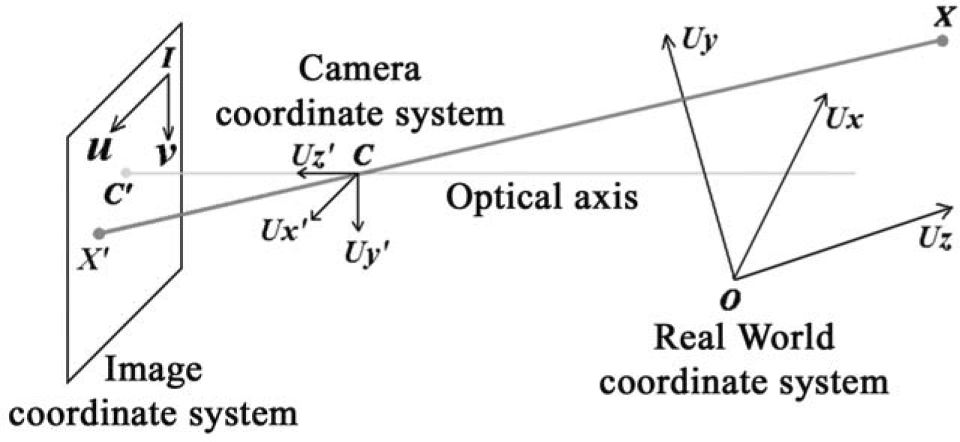
\includegraphics[width=9cm]{figs/pinholemodel.png}
\caption{Pin-hole model of a camera.}
\label{fig:pinholemodel}
\end{figure}

Some of the data types provided by this library are: \textit{HPoint2D} (to store a 2D point that usually belongs to the image plane), \textit{HPoint3D} (data point structure that represents a point in the 3D space) or \textit{TPinholeCamera} (pin-hole camera model defined by its extrinsics and intrinsics parameters).

And some of the functions which can be found are: \textit{project} (to project a 3D point on to the 2D image planer) and \textit{backproject} (to obtain the projection line that connects the camera with the focus and the 3D ray which is projected in a pixel of the image plane).

\subsubsection{Colorspaces}: espacios de color para imágenes

\subsubsection{Control template}
Basic component for reactive controllers



\subsubsection{VisualHFSM}
\subsubsection{Calibrator}
\subsubsection{ColorTuner}
\subsubsection{Recorder and replayer}

When we use real robots, one of the greatest difficulties is repeating experiments with the same conditions, whether we want to compare different algorithms or to test several features of the same algorithm. It's almost impossible to reproduce the same environment conditions, since robot hardware behaves diversely, light conditions change if we use cameras, people or objects move or are located in different places, etc.

To avoid all these matters, we have designed a new tool which records the current devices status and reproduces them whenever we want to. There are two components involved in this tool, the first one is the so-called "recorder", it saves in a file the status of all the devices of the robot, such as odometry, laser measures, image cameras, etc; we can configure which devices we want to track when we executes the components and it works with simulators, real Nao robots and real Pioneer robots.

The second components is the "replayer" component, it reads the file saved by the "recorder" component and provides the same ICE interfaces that would provide the real devices. Thus, when an algorithm gets the current devices status, it can't tell if it's obtaining the current devices measures in real time or pre-recorded data.

This tools has been widely used to perform experiments with real robots, to try different parameters and improve our algorithms.

\subsubsection{Android mobileTeleoperator}

Android operating system is increasing its market share every day, both with smartphones and tables. Once you develop an application for this platform, it may be used by students, other researchers or even companies. 

We have created an application called "Mobile Teleoperator" to teleoperate either a Pioneer robot with playerserver or a Nao Robot with BICA architecture. Connection among the mobile device and the robots is made through ICE, the same way we do when we use a standard computer, so we don't need to change anything in Jderobot architecture.

There are three ways to teleoperate the robots:
- Arrows: After pressing a button, it sends the command to the robot and the robot keeps his behavior until the stop button is pressed.
- Joystick: While a button is pressed, it send the command to the robot, but if the button is released it sends a stop command automatically.
- Accelerometer: It uses the mobile accelerometers to command the robot depending on our device orientation. To use this behavior you must keep a "safety" button pressed, this button is used to calibrate the accelerometers when it is pressed the first time and to send a stop command automatically once this button is released.

Mobile teleoperator has been used to create demonstrations and to let people who are not used to control robot to teleoperate robots in a easy way.


\subsubsection{KinectServer, openniServer and kinectViewer}
Kinect is one of the latest generation device more used in the last months. That is why jderobot icludes some components to support this device and allows to access to all the information that it provides. Through jderobot you can access to color, depth and IR values, and also to the tilt motor device and it leds.

Jderobot has two kinect servers that give us the possibility to access the sensor: kinectServer and openniServer. The main difference between this two components is the way to access to the device. KinectServer use PCL to access the sensor using the opennni\_grabber integrated on this library, whereas openniServer uses OpenNi directly preserving all the functionality of this framework. 

Although the servers access information in a different way both offer information using the same ICE interfaces so both components are completly compatible. 

The third component, kinectViewer, is able to connect to one of the servers below and to analyse  the information. This component integrates some of the 3D tools that jderobot provides and can represent the 3D information and reconstruct the scenario in an OpenGL world. 


\section{Research and Teaching}
\label{ref:research}

\subsection{Teaching robotics with Jderobot}

In an effort to stimulate young people to get involved with technology, robots seem a topic that attracts interest.

When allowing students to design, build and program their own robots, they will get involved in many technical activities that also overlap with several other disciplines like Mathematics, Engineering, Electronics, Information Technology and Science in general.

Also they will learn to work in teams and will be faced with many difficult technical decisions which enhance their management skills.

When setting up lessons there always is a challenge about how complicated the lessons should be. Special Jderobot components have been developed for students, in which a number of pre-programmed instructions are used to let students construct their own applications.

Such an approach eliminates the need to know a lot about gears, motors, using sensors, calibration and allows students to have a working robot within little over an hour.

The most important issue with the project is of course to interest students to get involved with technology. So it must be made very simple and yet interesting. It is very important that students can get their first results quickly, so they learn that they can master working with robots. This approach seems to facilitate this.


Starting with a basic component like Introrob is very stimulating. Once the enthusiasm has been generated, they still need to learn about motors, sensors, control issues and programming.

So it becomes important to offer a migration path from this very simple starting level to an environment where more skills are required. The best way is to start with a simple level and have a programming environment, such as Jderobot, that supports working from the very simple to a slightly more advanced level.


Having an integrated simulator is very important, so the students may quickly test their experiments without the need for a robot for every student. Such an environment is provided by The Player Project\footnote{http://playerstage.sourceforge.net/index.html}. This Open Source software is capable of simulating a population of robots, sensors and objects, but does so in a three-dimensional world.


\subsection{Robot navigation}

Obstacle avoidance is one of the key issues to successful applications of mobile robot systems. All mobile robots feature some kind of collision avoidance. It needs to steer the robot around the obstacle and proceed toward the original target.

We have implemented two famous navigation algorithms: VFF, as a obstacle avoidance or local path planning mechanism; and GPP, as a global path planner algorithm.

The Virtual Force Field (VFF) method is our earlier real-time obstacle avoidance method for our running robots. This technique allows for fast, continuous, and smooth motion of the controlled vehicle among unexpected obstacles, and does not require the vehicle to stop in front of obstacles.

On the other hand, when a trap-situation is flagged, the robot slows down (and may come to a complete halt),
while the VFF algorithm is temporarily suspended. The GPP algotirhm is then invoked to plan a new path based on the available information in the gradient field that represents the optimal (lowest-cost) path to the goal at every point in the workspace (see Figure {fig:gppNav}).

\begin{figure}
  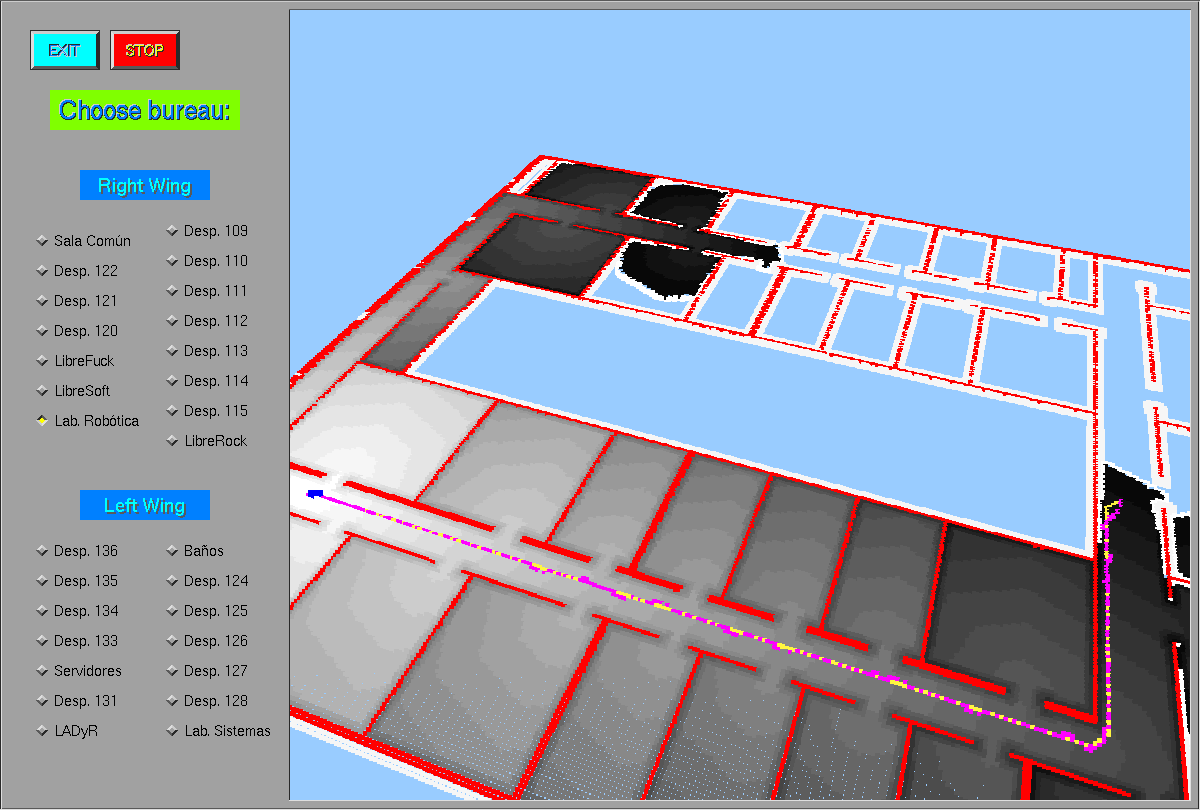
\includegraphics[width=9cm]{figs/gppNav.png}
\caption{Robot navigation using GPP and VFF algorithms.}
\label{fig:gppNav}
\end{figure}

Both techniques, VFF and GPP, have been implemented under Jderobot and extensively tested on Player-Stage and Gazebo simulators and on-board an ActivMedia Pioneer mobile robot, equipped with a ring of 24 ultrasonic sensors, and also using laser sensors, such as Hokuyo or Sick laser.

Follow person \cite{canas05d}.

\subsection{Evolutive Selflocalization algorithms}

Self-localization is at the moment one of the most important challenges in robotics. Using robot sensors, such as cameras, laser sensors or ultrasonic sensors, our robot must be able to calculate its own localization inside an environment. Once the robot knows its position, it can adapt its behavior depending on where it is located. 
 
However, robot self-localization has proven to be one the most complex task on mobile robots, since they must face unknown situations, such as occlusions, or being located inside a dynamic environment.

With Jderobot, we have designed and implemented plenty of localization algorithm, since classical localization algorithms such as Monte Carlo particle filters or Kalman filters, to new and improved algorithms such as evolutionary algorithms or MonoSLAM.

\subsection{MonoSLAM}

Monocular Simultaneous Localization And Mapping (MonoSLAM) is a type of localization first presented by Andrew J. Davison in 2003 (ref). MonoSLAM is able to construct a point-based map of the environment with a single camera, and localizates the camera inside this environment in real time.

We have developed our own MonoSLAM approach, based on Davison work, obtaining images from real cameras and simulators. We have implemented the point-based approach designed by Andrew Davison and afterwards we have designed our own implementations based on points and lines.

This type of localization is more accurate than classical localization methods and is very useful when robot odometry is not available or is not reliable. On the other hand, it is not able to handle occlusions and needs a faster frame rate.

% For two-column wide figures use
\begin{figure*}
% Use the relevant command to insert your figure file.
% For example, with the graphicx package use
  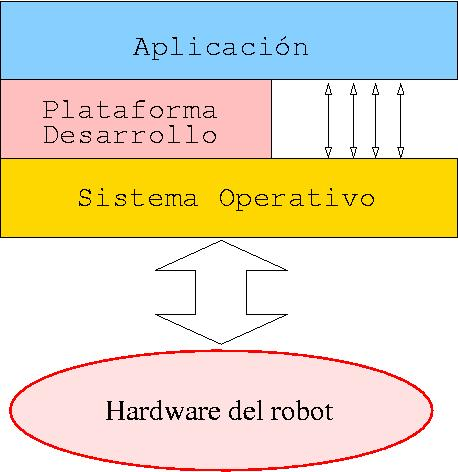
\includegraphics[width=7cm]{figs/programacion3.jpg}
% figure caption is below the figure
\caption{Please write your figure caption here}
\label{fig:2}       % Give a unique label
\end{figure*}

\section{Study about the Jderobot community}

%history
The Jderobot project started in 2003 as PhD thesis, as the software implementation of a cognitive architecture to develop autonomous behaviors in robots \cite{canas02,canas05e}. It provided access to robot camera, encoders, sonar sensors and motors using sockets between some drivers and the control application. The application was divided in \textit{schemas} implemented as concurrent threads. Its development was opened to a group of students. Several alternatives and expansions have been programmed \cite{canas07,canas07f}.

%current release
A major revision was undergone in 2010, leaving out the cognitive aspects and focusing in jderobot as a software architecture for robot applications. The major design principles followed has been described in section \ref{sec:jderobot}. The most recent release is 5.0. Currently it has a total of 123.531 lines of source code.

\begin{verbatim}
SLOC    Directory       SLOC-by-Language 
60707   src_components  cpp=32504,ansic=26370,
                        java=1355,xml=332,
                        sh=89,python=57
27509   src_interfaces  cpp=27509
23620   share           xml=23620
11354   src_libs        cpp=9979,ansic=1375
338     debian          sh=338
3       scripts         sh=3
\end{verbatim}

Totals grouped by language (current version of jderobot)
\begin{verbatim}
cpp:          69992 (56.66%)
ansic:        27745 (22.46%)
xml:          23952 (19.39%)
java:          1355 (1.10%)
sh:             430 (0.35%)
python:          57 (0.05%)
\end{verbatim}


\begin{figure}
  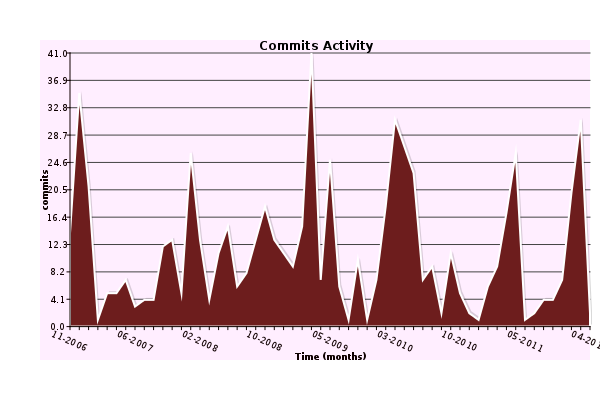
\includegraphics[width=7cm]{figs/svn_activity.png}
\caption{Activity of commits in the project}
\label{fig:svn-activity}
\end{figure}

\begin{figure}
  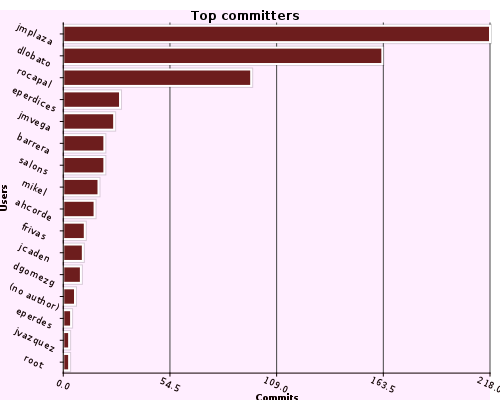
\includegraphics[width=7cm]{figs/svn_top-committers.png}
\caption{Top committers of Jderobot project}
\label{fig:svn-topcommiters}
\end{figure}

%who is using Jderobot
The users community includes the Robotics Group at Universidad Rey Juan Carlos, where it has been used in research and teaching. It also includes Universidad de Málaga, Universidad Carlos III and Politécnico Colombiano Jaime Cadavid.

%lessons learnt
High rotation in developers. Typically one student. Took a snapshot of Jderobot and developed its own extensions for her Final Degree Project. ---> Single repository. 2006. Web server, mediawiki for documentation.

The opening of the development.

\section{Conclusions}

Jderobot, open source project
\begin{itemize}
\item Más de 60000 líneas de código
\item Comunidad de usuarios y desarrolladores
%\item Aumentar la calidad del software
\item ¿Dónde conseguirla? ¿Cómo preguntar dudas? 
\item Página web: {http://jderobot.org}
\item Listas de correo: jde-users@gsyc.es y jde-developers@gsyc.es
\item Svn, trac, blog, mediawiki
\item Paquete debian: \texttt{apt-get install jderobot}
\end{itemize}

\begin{acknowledgements}
Funding agencies. Alex, Maikel, Fran.
\end{acknowledgements}

% BibTeX users please use one of
\bibliographystyle{spbasic}      % basic style, author-year citations
%\bibliographystyle{spmpsci}      % mathematics and physical sciences
%\bibliographystyle{spphys}       % APS-like style for physics
\bibliography{bibliografia}   % name your BibTeX data base


\end{document}


